\documentclass{article}\usepackage[]{graphicx}\usepackage[]{color}
%% maxwidth is the original width if it is less than linewidth
%% otherwise use linewidth (to make sure the graphics do not exceed the margin)
\makeatletter
\def\maxwidth{ %
  \ifdim\Gin@nat@width>\linewidth
    \linewidth
  \else
    \Gin@nat@width
  \fi
}
\makeatother

\definecolor{fgcolor}{rgb}{0.345, 0.345, 0.345}
\newcommand{\hlnum}[1]{\textcolor[rgb]{0.686,0.059,0.569}{#1}}%
\newcommand{\hlstr}[1]{\textcolor[rgb]{0.192,0.494,0.8}{#1}}%
\newcommand{\hlcom}[1]{\textcolor[rgb]{0.678,0.584,0.686}{\textit{#1}}}%
\newcommand{\hlopt}[1]{\textcolor[rgb]{0,0,0}{#1}}%
\newcommand{\hlstd}[1]{\textcolor[rgb]{0.345,0.345,0.345}{#1}}%
\newcommand{\hlkwa}[1]{\textcolor[rgb]{0.161,0.373,0.58}{\textbf{#1}}}%
\newcommand{\hlkwb}[1]{\textcolor[rgb]{0.69,0.353,0.396}{#1}}%
\newcommand{\hlkwc}[1]{\textcolor[rgb]{0.333,0.667,0.333}{#1}}%
\newcommand{\hlkwd}[1]{\textcolor[rgb]{0.737,0.353,0.396}{\textbf{#1}}}%

\usepackage{framed}
\makeatletter
\newenvironment{kframe}{%
 \def\at@end@of@kframe{}%
 \ifinner\ifhmode%
  \def\at@end@of@kframe{\end{minipage}}%
  \begin{minipage}{\columnwidth}%
 \fi\fi%
 \def\FrameCommand##1{\hskip\@totalleftmargin \hskip-\fboxsep
 \colorbox{shadecolor}{##1}\hskip-\fboxsep
     % There is no \\@totalrightmargin, so:
     \hskip-\linewidth \hskip-\@totalleftmargin \hskip\columnwidth}%
 \MakeFramed {\advance\hsize-\width
   \@totalleftmargin\z@ \linewidth\hsize
   \@setminipage}}%
 {\par\unskip\endMakeFramed%
 \at@end@of@kframe}
\makeatother

\definecolor{shadecolor}{rgb}{.97, .97, .97}
\definecolor{messagecolor}{rgb}{0, 0, 0}
\definecolor{warningcolor}{rgb}{1, 0, 1}
\definecolor{errorcolor}{rgb}{1, 0, 0}
\newenvironment{knitrout}{}{} % an empty environment to be redefined in TeX

\usepackage{alltt}
\usepackage{graphicx, color, amssymb, amsmath, bm, rotating, graphics,
epsfig, multicol, amsthm}
\usepackage{fullpage}
\usepackage[maxfloats=48]{morefloats} %for >18 figures
\usepackage{booktabs}
\usepackage{caption}
\usepackage[authoryear]{natbib}
%Independent: use as X \ind Y | Z
\newcommand\ind{\protect\mathpalette{\protect\independenT}{\perp}}
\def\independenT#1#2{\mathrel{\rlap{$#1#2$}\mkern2mu{#1#2}}}
\newtheorem{alg}{Algorithm}
\newtheorem{theorem}{Theorem}
\IfFileExists{upquote.sty}{\usepackage{upquote}}{}
\begin{document}




\title{Ancillarity-Sufficiency or not; Interweaving to improve MCMC estimation of the DLM}

\author{Matthew Simpson\textsuperscript{1}, Jarad Niemi\textsuperscript{2}, Vivekananda Roy\textsuperscript{2}}

\maketitle

\begin{center}
\small{---------------------------------------------------------------------------------------------------
\\
\textit{Second Bayesian Young Statisticians Meeting (BAYSM 2014)\\
Vienna,  September 18--19, 2014}
\\[-.3em]
---------------------------------------------------------------------------------------------------}
\end{center}

\begin{center}
 \vspace{-.5em}
 {\small \textsuperscript{1} Iowa State University, Depts. of Statistics and Economics, Ames, IA, USA\\[-.3em]
 {\tt simpsonm@iastate.edu}}
 
 \vspace{.5em}

{\small \textsuperscript{2} Iowa State University, Dept. of Statistics, Ames, IA, USA\\[-.3em]
{\tt <niemi,vroy>@iastate.edu}}

\end{center}

\vspace*{0.5em}

\begin{abstract}

In dynamic linear models (DLMs), MCMC sampling can often be very slow for estimating the posterior density --- especially for longer time series. In particular, in some regions of the parameter space the standard data augmentation algorithm can mix very slowly. Using some of the insights from the data augmentation for multilevel models literature, we explore several alternative data augmentations for a general class of DLMs and we show that no ``practical'' sufficient augmentation exists. In addition, we utilize these augmentations to construct several interweaving algorithms --- though we cannot construct an ancillary-sufficient interweaving algorithm (ASIS) since no sufficient augmentation exists, we find two ancillary augmentation and are able to construct a componentwise interweaving algorithm that uses ASIS for each model parameter conditional on the rest. Using the local level DLM, we show how to construct several of these algorithms and conduct a simulation study in order to discern their properties. We find that several algorithms that outperform the usual ``state sampler'' for many values of the population parameters, though there is room for improvement because one or more steps of the more efficient algorithms involves an often inefficient rejection sampling draw from a class of density that contains the generalized inverse Gaussian as a special case.

\textbf{Keywords}: data augmentation; time series; interweaving
\end{abstract}


\section{Introduction}
In dynamic linear models (DLMs), MCMC sampling can often be very slow for estimating the posterior density --- especially for longer time series. In particular, in some regions of the parameter space the standard data augmentation algorithm can mix very slowly. Using some of the insights from the data augmentation for multilevel models literature, we explore several alternative data augmentations for a general class of DLMs. The generic DLM can be defined as follows:
\begin{align}
  y_t &= F_t\theta_t + v_t && v_t \stackrel{ind}{\sim} N_k(0,V) \label{dlmtdobseq}\\
  \theta_t &= G_t\theta_{t-1} + w_t && w_t \stackrel{ind}{\sim} N_p(0,W) \label{dlmtdsyseq}
\end{align}
for $t=1,2,\cdots,T$, and $v_{1:T}$, $w_{1:T}$ independent. Equation \eqref{dlmtdobseq} is called the {\it observation equation} and equation \eqref{dlmtdsyseq} is called the {\it system equation}. Similarly, $v_{1:T}$ are called the {\it observation errors}, $V$ is called the {\it observation variance}, $w_{1:T}$ are called the {\it system disturbances} and $W$ is called the {\it system variance}. The observed data is $y_{1:T}$ while $\theta_{0:T}$ is called the latent states, and is the usual DA for this model. For each $t=1,2,\cdots,T$, $F_t$ is a $k\times p$ matrix and $G_t$ is a $p\times p$ matrix. Let $\phi$ denote the vector of unknown parameters in the model. Then possibly $F_{1:T}$, $G_{1:T}$, $V$, and $W$ are all functions of $\phi$, but we will assume $\phi=(V,W)$. To complete the model specification in a Bayesian context, we need priors on $\theta_0$, $V$, and $W$. We'll use the standard approach and assume that they are mutually independent a priori and that $\theta_0 \sim N(m_0, C_0)$, $V \sim IW(\Lambda_V, \lambda_V)$ and $W \sim IW(\Lambda_W, \lambda_W)$ where $m_0$, $C_0$, $\Lambda_V$, $\lambda_V$, $\Lambda_W$, and $\lambda_W$ are known hyperparameters and $IW(\Lambda, \lambda)$ denotes the inverse Wishart distribution with degrees of freedom $\lambda$ and positive definite scale matrix $\Lambda$.

\section{Results for the General DLM}

The standard method of estimating this model is via data augmentation (DA), as in \citet{fruhwirth1994data} and \citet{carter1994gibbs}. The basic idea is to implement a Gibbs sampler with two blocks. The generic DA algorithm with parameter $\phi$, augmented data $\theta$, and data $y$ obtains the $k+1$'st state of the Markov chain, $(\phi^{(k+1)},theta^{(k+1)})$, from the $k$'th state, $\phi^{(k)}$ as follows:
\begin{alg}DA algorithm.\label{alg:DA}\\
  \begin{center}
    \begin{tabular}{lll}
      $[\theta|\phi^{(k)}]$& $\to$& $[\phi^{(k+1)}|\theta]$.
    \end{tabular}
  \end{center}
\end{alg}
We construct two more data augmentations, the scaled disturbances, given by $\gamma_0=\theta_0$ and $\gamma_t = L_W^{-1}(\theta_t-G_t\theta_{t-1})$ for $t=1,2,\cdots,T$ where $L_W$ is the Cholesky factor of $W$, and the scaled errors, given by $\psi_0=\theta_0$ and $\psi_t=L_V^{-1}(y_t - F_t\theta_t)$ for $t=1,2,\cdots,T$ where $L_V$ is the Cholesky factor of $V$. The scaled disturbances are well known in the time series and multilevel models literature, e.g. \cite{fruhwirth2004efficient}, \citet{papaspiliopoulos2007general}, and \citet{van2001art}, as the ``non-centered augmentation'' but the scaled errors are novel. Both DAs are ancillary augmentations (AAs) --- generic DA $\theta$ is an AA if $p(\theta|\phi)=p(\phi)$ where $\phi$ is the model parameter. If we can find a sufficient augmentation (SA), i.e. a DA $\theta$ such that $p(y|\theta,\phi)=p(y|\theta)$ where $y$ is the data, then we can construct an ancillary--sufficient interweaving algorithm (ASIS) from \citet{yu2011center}. We show that any SA would be impractical to use, but nevertheless construct several interweaving algorithms including GIS and CIS algorithms. A GIS algorithm, or general interweaving strategy, based on two DAs $\theta$ and $\gamma$ has the form
\begin{alg}GIS Algorithm.\label{alg:GIS}\\
  \begin{center}
    \begin{tabular}{lllllll}
      $[\theta|\phi^{(k)}]$& $\to$& $[\phi|\theta]$& $\to $&$[\gamma|\theta,\phi]$& $\to$& $[\phi^{(k+1)}|\gamma]$
    \end{tabular}
  \end{center}
\end{alg}
while a CIS algorithm, or componentwise interweaving strategy, essentially runs a GIS step for $\phi_1$ given $\phi_2$ and a separate GIS step for $\phi_2|\phi_1$ where $\phi=(\phi_1,\phi_2)$. Much like the Gibbs sampler, this can be extended to multiple GIS steps and some of them may even be standard Gibbs steps. In particular, each GIS step can be an ASIS step when the two DAs used in that step form an AA-SA pair for $\phi_i|\phi_{-i}$. We show that the following CIS algorithm for the DLM is equivalent to a CIS algorithm with ASIS steps:
\begin{alg}Full CIS for DLMs, based on states.\label{alg:FCIS2}\\
  \begin{center}
    \begin{tabular}{llllllll}
      $[\theta_{0:T}|V^{(k)},W^{(k)}]$& $\to $& $[V|W^{(k)},\theta_{0:T}]$& $\to$& $[\psi_{0:T}|V,W^{(k)},\theta_{0:T}]$& $\to$& $[V^{(k+1)}|W^{(k)},\psi_{0:T}]$& $\to$\\
      $[\theta_{0:T}|V^{(k+1)},W^{(k)},\psi_{0:T}]$& $\to$& $[W|V^{(k+1)},\theta_{0:T}]$& $\to$& $[\gamma_{0:T}|V^{(k+1)},W,\theta_{0:T}]$& $\to$& $[W^{(k+1)}|V^{(k+1)},\gamma_{0:T}]$.
    \end{tabular}
  \end{center}
\end{alg}
Furthermore, we show that this algorithm is the same as the following Dist-Error GIS algorithm with some steps rearranged and $V$ and $W$ drawn separately instead of jointly:
\begin{alg}Dist-Error GIS for DLMs.\label{alg:Dist-Error}\\
  \begin{center}
    \begin{tabular}{llllllll}
      $[\gamma_{0:T}|V^{(k)},W^{(k)}]$& $\to $& $[V|W^{(k)},\gamma_{0:T}]$& $\to$& $[W|V,\gamma_{0:T}]$& $\to$\\
      $[\psi_{0:T}|V,W,\gamma_{0:T}]$& $\to$& $[V^{(k+1)}|W,\psi_{0:T}]$& $\to$& $[W^{(k+1)}|V^{(k+1)},\psi_{0:T}]$.&
    \end{tabular}
  \end{center}
\end{alg}

\section{Simulation Study in the Local Level Model}

We apply these algorithms in a worked example using the local level model where $G_t=F_t=1$ for $t=1,2,\cdots,T$ with one difference --- $V$ and $W$ are sampled separately instead of jointly when conditioning on the scaled disturbances or the scaled errors. In doing so, when we draw $W|V,\gamma_{0:T}$ or $V|W,\psi_{0:T}$, we draw from the following density
\begin{align*}
  p(x) \propto x^{-\alpha - 1}\exp\left[ -ax + b\sqrt{x}  -\beta/x\right]
\end{align*}
where $\alpha,a,\beta>0$ and $b\in \Re$. This density contains the generalized inverse Gaussian as a special case when $b=0$, but is difficult to sample from efficiently, which hurts any algorithm based on the ``scaled'' DAs. We use adaptive rejection sampling (\citet{gilks1992adaptive}) when possible, but otherwise use rejection sampler with a Cauchy proposal for $\log(x)$.

Using this worked example, we simulated a fake dataset from the local level model for various choices of $V$, $W$, and $T$. We created a grid over $V$--$W$ space with $(V,W)$ ranging from $(10^{-2},10^{-2})$ to $(10^2, 10^2)$ and we simulated a dataset for all possible combinations of $V$ and $W$ with each of $T=10, 100, 1000$. Then for each dataset, we fit the local level model using each DA algorithm, each GIS algorithm based on any two of the DAs, and the CIS algorithm. We used the same rule for constructing priors for each model: $\theta_0\sim N(0,10^7)$, $V\sim IG(5, 4V^*)$, and $W\sim IG(5, 4W^*)$, mutually independent where $(V^*,W^*)$ are the true values of $V$ and $W$ used to simulate the time series. So the prior mean is equal to the true values of $V$ and $W$ so that both the prior and likelihood and thus the posterior roughly agree about the likely values of $V$ and $W$. For each dataset and each sampler we obtained $n=3000$ draws and threw away the first $500$ as burn in. The chains were started at the true values used to simulated the time series, so we can examine the behavior of the chains to determine how well they mix but not how quickly they converge. We look at the effective sample size (ESS) (see e.g. \citet{gelman2003bayesian}) of each component component in order to assess the MCMC efficiency of each sampler. 

Table \ref{tab:stnmix} summarizes the results for each MCMC sampler. We find that the state sampler, the DA algorithm based on the states, has a high ESS for $V$ when the population signal-to-noise ratio $R=W^*/V^*$ is less than one, and a high ESS for $W$ when $R$ is greater than one. The scaled disturbance sampler has a high ESS for both $V$ and $W$ when $R<1$ while the scaled error sampler has a high ESS for both $V$ and $W$ when $R>1$. The GIS algorithms, i.e. State-Dist, State-Error, and Dist-Error, all have high ESS for either $V$ or $W$ when at least one of the two DA algorithms it is based on has a high ESS for that parameter, e.g. the Dist-Error algorithm has high ESS for both $V$ and $W$ as long as $R$ is not too close to one. The CIS algorithm behaves essentially identically to the Dist-Error algorithm. One major caveat to this table is that as $T$, the length of the time series, increases, all ESS's decrease so that e.g. for the Dist-Error sampler to have high ESS's for $V$ and $W$, $R$ must be farther and farther from one.

\begin{table}
  \centering
  \begin{tabular}{|l|ccccccc|}\hline
    Parameter & State & Dist & Error  & State-Dist        & State-Error       & Dist-Error        & Full CIS \\\hline
    V & $R < 1$ & $R < 1$ & $R > 1$ & $R < 1$           & $R \not\approx 1$ & $R \not\approx 1$ & $R \not\approx 1$ \\
    W & $R > 1$ & $R < 1$ & $R > 1$ & $R \not\approx 1$ & $R > 1$           & $R \not\approx 1$ &  $R \not\approx 1$\\\hline
  \end{tabular}
  \caption{Rule of thumb for when each algorithm has a high effective sample size for each variable as a function of the true signal-to-noise ratio, $R=W/V$.}
  \label{tab:stnmix}
\end{table}




Figure \ref{plot} contains a plot of the log time per 1000 effective draws, i.e.
\[
\log\frac{\mathrm{time\ in\ minutes}}{\mathrm{effective\ sample\ size}}.
\]
When computational time is taken into account, the Dist-Error GIS and Full CIS algorithms come out on top, despite both algorithms having to inefficiently draw from the density mentioned above. With a better method of drawing from these densities, these two samplers will improve even more.

\begin{knitrout}
\definecolor{shadecolor}{rgb}{0.969, 0.969, 0.969}\color{fgcolor}\begin{figure}[]


{\centering 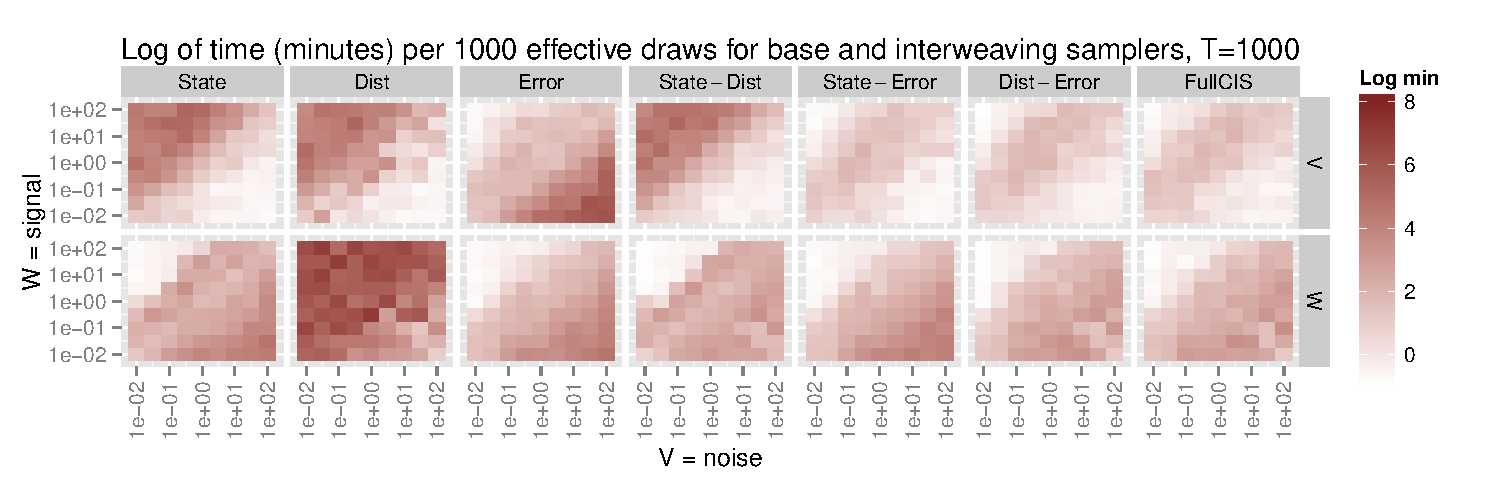
\includegraphics[width=.8\textwidth]{figure/plot} 

}

\caption[Log of the time in minutes per 1000 effective draws in the posterior sampler for $V$ and $W$, and for a time series of length $T=1000$ in the state, scaled disturbance and scaled error samplers and for all four interweaving samplers]{Log of the time in minutes per 1000 effective draws in the posterior sampler for $V$ and $W$, and for a time series of length $T=1000$ in the state, scaled disturbance and scaled error samplers and for all four interweaving samplers. Horizontal and vertical axes indicate the true values of $V$ and $W$ respectively for the simulated data. The signal-to-noise ratio is constant moving up any diagonal. In the upper left the signal is high, in the lower right the noise is high.\label{plot}}
\end{figure}


\end{knitrout}


\bibliographystyle{plainnat}
\bibliography{../mcmcex}
\end{document}
